\section{Введение}\label{sec:introduction}

Разрешение имён -- ключевая функция фронт-энда компилятора и современных сред разработки (IDE). Она применяется для перехода к определению, поддержки рефакторинга, семантической подсветки~\cite{Neron2015,vanAntwerpen2018}. На практике большинство реализаций остаётся привязано к конкретным языкам и носит характер ad hoc решений. Это затрудняет переносимость инструментов и построение формальных доказательств их корректности~\cite{vanAntwerpen2018,Zwaan2023}. В работах по графам областей видимости (Scope Graphs) предложена модель связывания имён, отделяющая структуру AST от правил построения графа областей видимости (Scope Graph) и семантики разрешения имён. Данная модель стала основой для декларативных спецификаций и реализации разрешения имён в коде~\cite{Neron2015,vanAntwerpen2018,Zwaan2023}. Для больших кодовых баз предложены стековые графы (Stack Graphs) с инкрементальным построением графа по файлам и стековым алгоритмом поиска определений~\cite{Creager2023}.

С точки зрения формализации и алгоритмов, многие задачи анализа программ сводимы к задаче КС-достижимости, лежащей в основе ряда межпроцедурных и иных анализов~\cite{RepsHorwitzSagiv1995,Hellings2015,HeLuXue2024}. Задача КС-достижимости состоит в поиске всех пар вершин в графе с метками на рёбрах, между которыми существует такой путь, что слово составленное из меток его рёбер принадлежит заданному контекстно-свободному языку. Есть основания полагать, что часть шаблонов разрешения имён также может быть сведена к задаче достижимости с контекстно-свободными ограничениями. Целью данной работы является повышение эффективности (выражаемой в меньших затратах по времени и по памяти) механизмов разрешения имён за счёт теоретического и практического исследования сводимости стековых графов к КС-достижимости.

\section{Стековые графы и КС-достижимость}\label{sec:models}

В качестве примера рассматривается следующий код на языке программирования Java:

\begin{figure}[htb]
\centering
\begin{minipage}[t]{0.44\textwidth}
\begin{Verbatim}[fontsize=\small]
# other.java
class Y {
    public int x;
    public Y() { this.x = 0; }
}
\end{Verbatim}
\end{minipage}
\hfill
\begin{minipage}[t]{0.50\textwidth}
\begin{Verbatim}[fontsize=\small]
# main.java
class HelloWorld {
    public static void main() {
        Y y;
        y.x;
    }
}
\end{Verbatim}
\end{minipage}
\caption*{\textbf{Листинг 1.} Пример исходного кода}
\label{lst:java-example}
\end{figure}

Пусть требуется разрешить ссылку на символ \(x\) в выражении \(y.x\) в \emph{main.java}. \(x\) является полем объекта \(y\), следовательно, необходимо сначала разрешить ссылку \(y\). Определение находится строкой выше и указывает, что \(y\) имеет тип \(Y\). Необходимо разрешить ссылку на символ \(Y\). Определение \(Y\) находится в файле \emph{other.java} и содержит определение \(x\), которое и является решением задачи.

Для формального обоснования предлагаемого метода вводятся определения стековых графов и задачи КС-достижимости.

\subsection{Стековые графы}\label{sec:stack-graphs}

Для решения задачи разрешения имён может применяться модель стековых графов.

Стековый граф \(G\) является представлением программы \(P\). Программа \(P\) состоит из множества файлов исходного кода \(F_{i}\). Каждый файл исходного кода представим в виде множества синтаксических вершин (вершин синтаксического древа). В данном множестве синтаксических вершин можно выделить два подмножества (возможно пересекающихся): подмножество вершин, отражающих определения, и подмножество вершин, отражающих ссылки в исходном коде.

Пусть символ \(x\) -- идентификатор из исходного кода, отражающий имя некой сущности в программе (или часть такого имени), либо символ оператора (например, оператор доступа к члену объекта \(.\) или оператор вызова \(()\)).

Каждая вершина стекового графа \(G\) принадлежит к одному из четырёх типов:

\begin{enumerate}
\def\labelenumi{\arabic{enumi}.}
\item
  Вершина области видимости (Scope node);
\item
  Корневая вершина (Root node);
\item
  Вершина добавления символа \(x\) на стек (Push node, далее вершина добавления);
\item
  Вершина удаления символа \(x\) со стека (Pop node, далее вершина удаления).
\end{enumerate}

Дополнительно, каждая вершина \(N_{i}\) кроме корневой относится ровно к одному файлу исходного кода \(F_{i}\). Часть вершин стекового графа \(G\) относится к конкретным синтаксическим вершинам данного файла \(F_{i}\). Вершина добавления \(N_{i}\) называется вершиной ссылки, если она относится к синтаксической вершине, отражающей ссылку. Вершина удаления \(N_{i}\) называется вершиной определения, если она относится к синтаксической вершине, отражающей определение.

Пусть \(E_{G}\) -- множество рёбер стекового графа \(G_{i}\). Каждое ребро стекового графа направлено и соединяет входную вершину \(N_{i}\) с выходной вершиной \(N_{i}'\). Рёбра могут соединять только вершины, принадлежащие одному файлу исходного кода \(F_{i}\)~\cite{Creager2023}.

Путь \(p\) в стековом графе \(G\) состоит из начальной вершины \(N_{i}\), конечной вершины \(N_{i}'\) и стека символов \(\widehat{x}\). Путь называется завершённым, если начальная вершина пути является вершиной ссылки, конечная вершина пути является вершиной определения и стек символов пути пуст. Каждое разрешение имени в программе \(P\) выразимо в виде завершённого пути в соответствующем данной программе стековом графе \(G\)~\cite{Creager2023}.

Пустым путём называется путь, не содержащий рёбер. Такой путь создаётся путём поднятия вершины стекового графа. Поднятие вершины добавления кладёт соответствующий ей символ \(x\) на стек символов. Вершина удаления не может быть поднята. Другие вершины дают пустой путь с пустым символьным стеком.

Любой путь \(p\) может быть расширен путём добавления к нему ребра \(E_{i}\), исходящего из конечной вершины данного пути \(p\). Выходная вершина \(N_{i}'\) этого ребра \(E_{i}\) становится новой конечной вершиной пути \(p\). Символьный стек пути \(p\) меняется в зависимости от новой конечной вершины \(N_{i}'\). Если вершина \(N_{i}'\) является корневой вершиной или вершиной области видимости, то стек символов \(\widehat{x}\) не меняется. Если вершина \(N_{i}'\) является вершиной добавления, то соответствующий ей символ \(x\) кладётся на стек символов \(\widehat{x}\). Если вершина \(N_{i}'\) является вершиной удаления, то расширение пути возможно только в том случае, когда стек символов \(\widehat{x}\) не пуст и на его вершине лежит символ \(x\), которому вершина удаления \(N_{i}'\) соответствует. В таком случае этот символ \(x\) снимается с вершины стека символов \(\widehat{x}\).

Если конечная вершина пути является корневой вершиной, то данный путь можно расширить до корневой вершины в подграфе любого другого файла (можно сказать, что корневая вершина принадлежит одновременно всем файлам). Это единственный способ проложить путь из одного файла в другой~\cite{Creager2023}.

На основе определения завершённого пути, способов создания пустого пути и способов расширения пути можно построить алгоритм разрешения имён в стековом графе.

Пусть дана программа \(P\) и ссылка в данной программе. Требуется найти все определения в программе \(P\), соответствующие данной ссылке.

Строится стековый граф \(G\), соответствующий программе \(P\). Пустой путь \(p\) создаётся поднятием вершины, соответствующей данной ссылке. Затем от этой вершины выполняется обход в ширину. Очередь ожидающих путей изначально содержит только \(p\). На каждом шаге следующий путь извлекается из очереди, после чего к нему поочерёдно добавляются рёбра, исходящие из его конечной вершины. Если добавление допустимо по описанным выше правилам, новый путь помещается в очередь. Если найденный путь завершён, его конечная вершина соответствует искомому определению~\cite{Creager2023}.

На рис.~\ref{fig:stack-graph} показан стековый граф для кода из листинга 1. Вершины помещения (\(push\)) и извлечения (\(pop\)) обозначают соответственно добавление указанного символа на вершину стека и снятие верхнего символа при совпадении. Вершины областей видимости (\(scope\)) представляют области видимости. Корневая вершина (\(root\)) обеспечивает переход между файловыми подграфами. Ориентированные рёбра задают допустимые продолжения пути. Символы «.» и «:» введены правилами построения графа для Java: «.» моделирует обращение к члену объекта, а «:» обозначает запрос типа выражения. Зелёным выделен завершённый путь, связывающий ссылку \(x\) в выражении \emph{y.x} с определением поля \(x\) класса \(Y\).

\begin{figure}[htb]
\centering
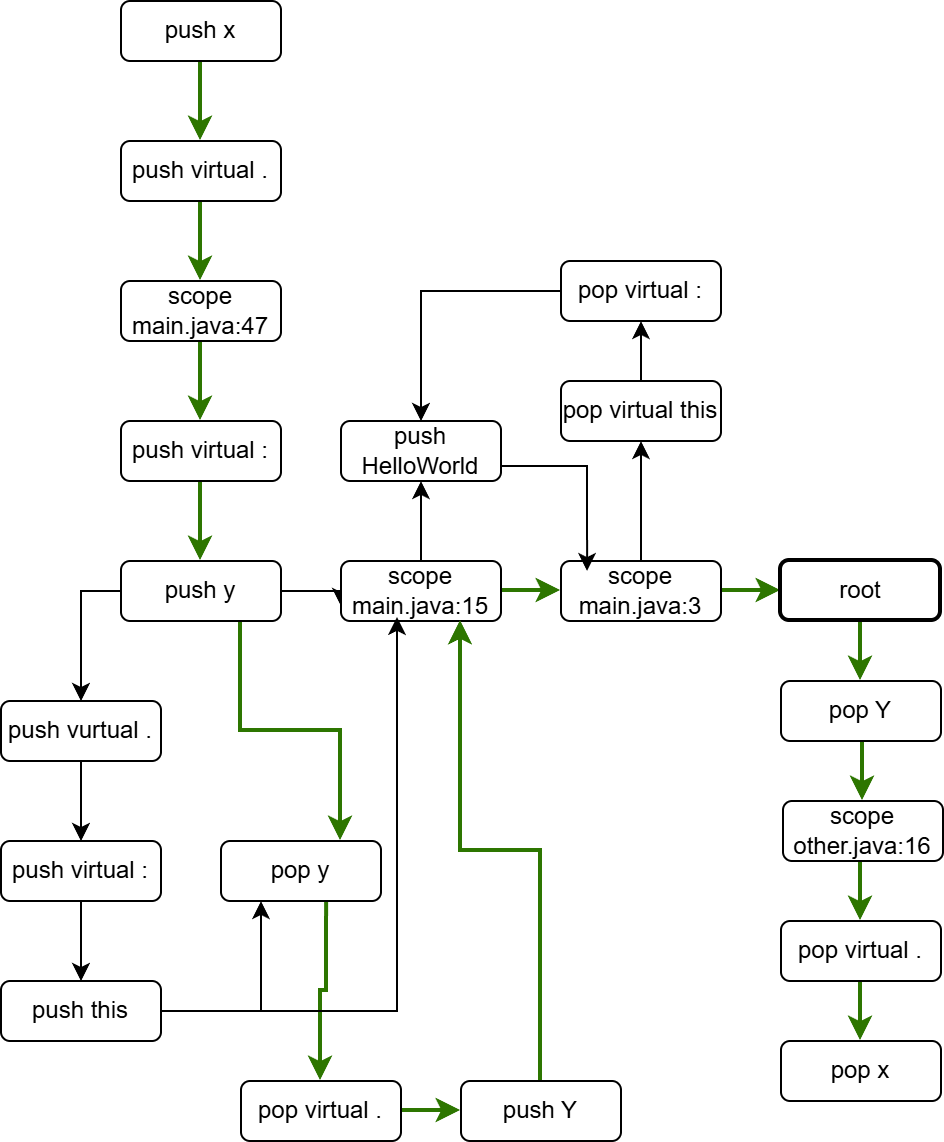
\includegraphics[width=0.72\textwidth]{figure1.png}
\caption{Пример стекового графа}
\label{fig:stack-graph}
\end{figure}

Граф строится из локальных фрагментов, создаваемых по правилам для синтаксических конструкций анализируемого языка (в нашем случае, для Java). Рёбра связывают эти фрагменты через вершины областей видимости в соответствии с правилами разрешения и вложенностью областей. Ссылка \(x\) в выражении \emph{y.x} образует начальную вершину \({push}_{x}\). Доступ к члену объекта добавляет внутреннюю вершину \({push}_{.}\) и направляет поиск к типу объекта \(y\). Для получения типа идентификатора правила Java создают переход через \({push}_{:}\) к ссылке \({push}_{y}\). Объявление \emph{Y y} представлено фрагментом \({pop}_{y}\  \rightarrow \ {pop}_{:}\  \rightarrow \ {push}_{Y}\). Вершина \({pop}_{y}\) сопоставляет ссылку с объявлением переменной, \({pop}_{:}\) завершает запрос её типа, а \({push}_{Y}\) начинает разрешение имени объявленного типа. Через области видимости файла \emph{main.java} и корневую вершину путь переходит в подграф файла \emph{other.java}, где \({pop}_{Y}\) сопоставляет имя типа с объявлением класса. Затем путь входит в область видимости членов класса: \({pop}_{.}\) снимает маркер обращения к члену, а \({pop}_{x}\) сопоставляет исходную ссылку с определением поля.

Зелёный путь показывает последовательность разрешения. Если вершину стека располагать слева, состояния символьного стека после операций \(push\) и \(pop\) имеют следующий вид:
\[
\begin{aligned}
\lbrack x\rbrack &\to \lbrack.,x\rbrack \to \lbrack:,.,x\rbrack
  \to \lbrack y,:,.,x\rbrack \to \lbrack:,.,x\rbrack \\
&\to \lbrack.,x\rbrack \to \lbrack Y,.,x\rbrack
  \to \lbrack.,x\rbrack \to \lbrack x\rbrack \to \lbrack\rbrack .
\end{aligned}
\]

Вершины областей видимости и корневая вершина стек не изменяют. Пустой стек после прохождения конечной вершины \({pop}_{x}\) показывает, что путь завершён и связывает ссылку \(x\) с определением поля \(x\) класса \(Y\).

Числа в вершинах областей видимости являются идентификаторами областей видимости данного файла. Граф на рис.~\ref{fig:stack-graph} визуально сокращён: на схеме показана часть вершин и рёбер полного графа, достаточная для разбора выделенного пути. Полный граф существенно больше из-за дополнительных вершин областей видимости и ответвлений.

\subsection{Задача КС-достижимости}\label{sec:cfl-reachability}

Задача КС-достижимости определяется тремя объектами: граф \(G\), алфавит \(\Sigma\) и контекстно-свободный язык \(L\), заданный над алфавитом \(\Sigma\).

Граф \(G\) состоит из множества вершин \(V\) и множества рёбер \(E\), где \(E\  \subseteq \ V\  \times \ (\Sigma\  \cup \ \{\varepsilon\})\  \times \ V\). Рёбра ориентированы и размечены символами алфавита \(\Sigma\) или меткой \(\varepsilon\). Символы алфавита далее называются терминалами.

Путь \(p\) в графе представлен последовательностью рёбер \(E_{1}\ \ldots\ E_{n}\). Пути \(p\) соответствует слово \(w_{p}\), образованное последовательной записью меток этих рёбер. Метка \(\varepsilon\) не добавляет символа в слово.

Пара вершин \((u,\ v)\) графа \(G\) называется КС-достижимой, если существует путь \(p\) из \(u\) в \(v\), слово которого принадлежит языку \(L\).

Решение задачи КС-достижимости сводится к нахождению всех КС-достижимых пар вершин \((u,\ v)\) графа \(G\)~\cite{MuravevGrigorev2025}.

\section{Сведение стековых графов к КС-достижимости}\label{sec:conversion}

В разделе дано формальное описание разработанного метода сведения, указана область его применимости и описано программное средство, созданное для демонстрации метода.

\subsection{Теоретическое описание сведения}\label{sec:conversion-theory}

Рассматривается конечный путь \(p_{S}\) = \((N_{1},\ \ldots,\ N_{n})\) в стековом графе \(G_{S}\). Операция, соответствующая начальной вершине, входит в слово пути. Если начальная вершина является вершиной-ссылкой, соответствующий символ помещается на стек.

Далее рассматривается модель, в которой допустимость пути определяется символьным стеком. Вершины областей видимости и корневая вершина этот стек не изменяют. Корневая вершина обеспечивает переход между файловыми подграфами.

Множество символов стекового графа обозначается \(X\  = \ \{ x_{i}\ |\ i\  \in \ I\}\). Вершине помещения символа \(x_{i}\) сопоставляется терминал \({push}_{i}\), а вершине извлечения того же символа сопоставляется терминал \({pop}_{i}\). Операция \({push}_{i}\) добавляет \(x_{i}\) к текущему стеку. Операция \({pop}_{i}\) допустима только при наличии \(x_{i}\) на вершине стека и удаляет этот символ. Слово пути образуется последовательностью этих операций. Нейтральные вершины не добавляют символов в слово пути.

Слова фрагментов пути, оставляющих символьный стек неизменным, описывает нетерминал \(S\):

\[S \to \varepsilon \mid S\,S \mid {push}_{i}\,S\,{pop}_{i},\qquad i \in I.\]

Для запросов разрешения имён, рассматриваемых далее, используется стартовый нетерминал \(Q\):

\[Q \to {push}_{i}\,S\,{pop}_{i},\qquad i \in I.\]

Эти правила задают контекстно-свободный язык \(L_{S}\). Правило \(S\  \rightarrow \ S\ S\) допускает произвольное число последовательных согласованных фрагментов, а правило с одинаковым индексом \(i\) обеспечивает правильную вложенность операций. К терминалам относятся только \({push}_{i}\) и \({pop}_{i}\). Обозначения \(S\) и \(Q\) являются нетерминалами, а \(\varepsilon\) обозначает пустое слово.

Пусть \(R\) и \(D\) обозначают множества вершин-ссылок и вершин-определений. При сведении каждой вершине \(r\  \in \ R\) сопоставляется вход \(r_{in}\). Каждой вершине \(d\  \in \ D\) сопоставляется выход \(d_{out}\). В построенной задаче КС-достижимости пара \((r,\ d)\) считается результатом запроса, если существует путь из \(r_{in}\) в \(d_{out}\), слово которого выводится из стартового нетерминала \(Q\).

В математической записи \(\varepsilon\) обозначает пустое слово. Ребро с меткой \(\varepsilon\) является нейтральным. Прохождение такого ребра не добавляет терминала в слово пути и не изменяет символьный стек.

При преобразовании обозначения \({push}_{i}\) и \({pop}_{i}\) переносятся с вершин на рёбра. Преобразование выполняется следующим образом.

\begin{enumerate}
\def\labelenumi{\arabic{enumi}.}
\item
  Вершинам помещения и извлечения сопоставляются метки \({push}_{i}\) и \({pop}_{i}\). Вершины областей видимости и корневая вершина остаются нейтральными.
\item
  На промежуточном этапе метки могут находиться как на вершинах, так и на рёбрах графа. Нейтральные элементы не добавляют символов в слово пути.
\item
  Все исходные рёбра получают нейтральную метку \(\varepsilon\). Прохождение такого ребра не изменяет слово пути.
\item
  Нейтральные метки удаляются с вершин областей видимости и с корневой вершины. Удаление этих меток не изменяет слова путей.
\item
  Каждая вершина с меткой \({push}_{i}\) заменяется парой вершин без меток \(N_{in}\) и \(N_{out}\). Входящие рёбра перенаправляются в \(N_{in}\). Исходящие рёбра перенаправляются из \(N_{out}\). Между \(N_{in}\) и \(N_{out}\) добавляется ребро с меткой \({push}_{i}\). Каждому исходному пути через заменяемую вершину соответствует единственный путь через созданную пару с той же операцией в той же позиции слова. Если исходная вершина была вершиной ссылки, \(N_{in}\) становится соответствующим входом \(r_{in}\).
\item
  Аналогично заменяются вершины с меткой \({pop}_{i}\). Если исходный путь заканчивался в вершине-определении, преобразованный путь заканчивается в соответствующей вершине \(N_{out}\), которая служит выходом \(d_{out}\).
\end{enumerate}

После преобразования обозначения \({push}_{i}\) и \({pop}_{i}\) существуют только как метки рёбер. Нейтральные рёбра имеют метку \(\varepsilon\). Алфавит терминалов состоит из \({push}_{i}\) и \({pop}_{i}\). Время построения графа составляет \(O(|V|\  + \ |E|)\), поскольку каждая вершина и каждое ребро обрабатываются постоянное число раз.

Псевдокод описанного алгоритма:

\begin{Verbatim}[fontsize=\small]
fn stack_graph_to_cfl(G: Graph) -> Graph:
    for node in G.nodes:
        # Push(x) -> push_x, Pop(x) -> pop_x,
        # Root and Scope -> epsilon
        node.label = make_node_label(node)
    for edge in G.edges:
        edge.label = epsilon
    for node in G.nodes where node.label == epsilon:
        delete node.label
    for node in G.nodes where node.label is push_*:
        let (N_in, N_out) = G.create_nodes_pair()
        redirect_incoming_edges(old_dest: node, new_dest: N_in)
        redirect_outgoing_edges(old_src: node, new_src: N_out)
        G.create_edge(N_in, N_out, label: node.label)
        if G.start_node == node:
            G.start_node = N_in
        G.delete_node(node)
    # То же самое для pop-вершин
    return G
\end{Verbatim}

Пример замены вершины помещения приведён на рис.~\ref{fig:push-before} и~\ref{fig:push-after}.

\setcounter{figure}{2}
\begin{figure}[htb]
\centering
\begin{minipage}[t]{0.46\textwidth}
\centering
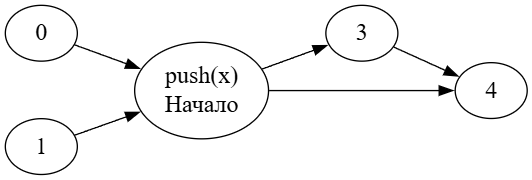
\includegraphics[width=\linewidth]{figure3.png}
\captionof{figure}{Вершина помещения до преобразования}
\label{fig:push-before}
\end{minipage}
\hfill
\begin{minipage}[t]{0.48\textwidth}
\centering
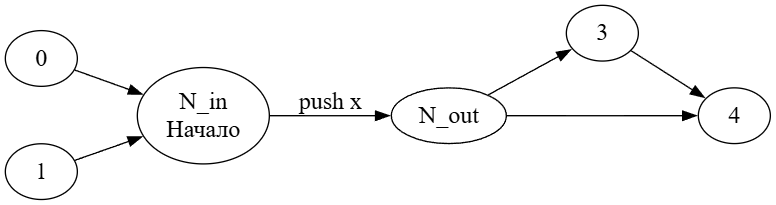
\includegraphics[width=\linewidth]{figure4.png}
\captionof{figure}{Вершина помещения после преобразования}
\label{fig:push-after}
\end{minipage}
\end{figure}

При разрешении всех ссылок рассматриваются входы \(r_{in}\), соответствующие вершинам-ссылкам. В результат включаются все пары \((r,\ d)\), для которых существует путь из \(r_{in}\) в \(d_{out}\), слово которого выводится из стартового нетерминала \(Q\).

На рис.~\ref{fig:converted-graph} показан результат сведения графа с рис.~\ref{fig:stack-graph}. Каждая вершина помещения или извлечения заменяется парой вершин \(N_{in}\) и \(N_{out}\) без меток, соединённых ребром с меткой соответствующей операции. Входящие рёбра перенаправляются в \(N_{in}\). Исходящие рёбра перенаправляются из \(N_{out}\). Вершины областей видимости и корневая вершина сохраняются, а исходные рёбра стекового графа получают нейтральную метку \(\varepsilon\). Преобразование сохраняет разветвления, порядок прохождения и последовательность операций пути.

\begin{figure}[htb]
\centering
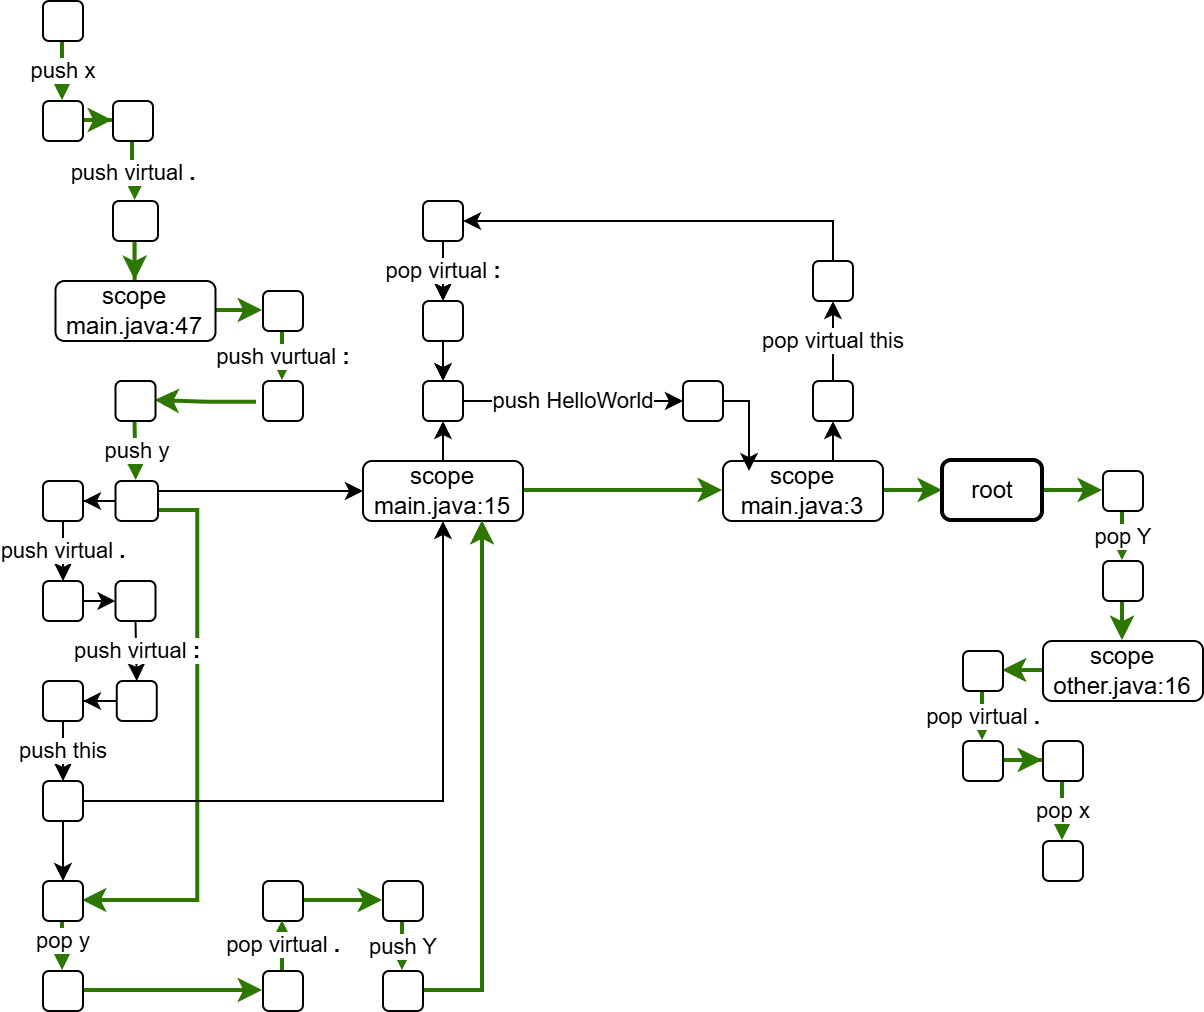
\includegraphics[width=0.90\textwidth]{figure5.png}
\caption{Результат сведения стекового графа из рис.~\ref{fig:stack-graph}}
\label{fig:converted-graph}
\end{figure}

Зелёный путь на рис.~\ref{fig:converted-graph} соответствует зелёному пути на рис.~\ref{fig:stack-graph}. Если опустить нейтральные рёбра, его слово имеет вид

\[
\begin{aligned}
{push}_{x} &\to {push}_{.} \to {push}_{:} \to {push}_{y} \to {pop}_{y} \\
&\to {pop}_{:} \to {push}_{Y} \to {pop}_{Y} \to {pop}_{.} \to {pop}_{x}.
\end{aligned}
\]

Операции вложены и попарно согласованы: каждая операция \(pop\) снимает верхний совпадающий символ, поэтому слово выводится из \(Q\). Вершина \(N_{in}\) пары, заменившей \({push}_{x}\), соответствует исходной ссылке, а вершина \(N_{out}\) пары, заменившей \({pop}_{x}\), соответствует определению. Тем самым сведение сохраняет связь ссылки \(x\) в выражении \emph{y.x} с определением поля \(x\) класса \(Y\).

\subsection{Программное средство StackGraphExporter}\label{sec:exporter}

Для практической реализации описанного выше сведения стековых графов к задаче КС-достижимости разработана утилита командной строки StackGraphExporter~\cite{CoreJustStackGraphExporter} на языке Rust. Программное средство строит стековые графы по файлам исходного кода, выполняет запросы разрешения на стековом графе, сводит стековые графы к задаче КС-достижимости, при необходимости упрощает граф в процессе сведения и создаёт артефакты для последующего запуска внешних решателей.

В экспериментах библиотека stack-graphs 0.14.1 используется как эталонная реализация. Перед выполнением запросов библиотека для каждого файла строит минимальный набор частичных путей и помещает его в базу. Частичный путь представляет собой фрагмент пути разрешения, который можно состыковать с другими фрагментами. При разрешении ссылки библиотека объединяет совместимые частичные пути в полные пути от ссылки к определениям.

\section{Результаты экспериментов}\label{sec:experiments}

Для проверки корректности реализации сведения и измерения эффективности разработанного программного средства проведена серия экспериментов. В разделе приведены постановка экспериментов и результаты.

\subsection{Постановка экспериментов}\label{sec:experiment-setup}

В эксперименте отобраны четыре проекта на Java с платформы GitHub: libgdx~\cite{LibGDX}, Shattered Pixel Dungeon~\cite{ShatteredPixelDungeon}, JsonPath~\cite{JaywayJsonPath} и JiaoZi Video Player~\cite{JiaoZiVideoPlayer}. В качестве внешнего решателя использовался CFG\_bench. В рамках каждого эксперимента выполнено 10 запусков. Средние значения времени запроса и потребляемой памяти рассчитаны средствами решателя. Для stack-graphs перед измерениями выполнялись два разогревочных запуска, а среднее значение рассчитывалось по пяти последующим запускам. Пиковое потребление ОЗУ в таблице приведено отдельно для stack-graphs и CFG\_bench. Показатель для stack-graphs измерялся с помощью библиотеки peak\_alloc. В каждом случае выполнялось разрешение всех ссылок в графе. Техническое окружение: ноутбук под управлением Windows 11 Pro, процессор AMD Ryzen 9 8940HX, 32 ГБ ОЗУ DDR5 SDRAM.

\subsection{Проверка корректности}\label{sec:correctness}

Для проверки корректности реализации сведения стекового графа к задаче КС-достижимости использовался решатель CFG\_bench. В результате решения задачи КС-достижимости определялось количество найденных пар вершин. Полученное значение сравнивалось с количеством пар, найденных при запросах в стековом графе.

\subsection{Результаты для запроса всех ссылок в графе}\label{sec:all-references}

Результаты экспериментов приведены в табл.~\ref{tab:results}.

\begin{table}[H]
\centering
\caption{Результаты выполнения запросов для всех пар}
\label{tab:results}
\scriptsize
\begin{tblr}{
  width=\textwidth,
  colspec={X[2.05,l] X[0.95,c] X[1.10,c] X[0.95,c] X[1.10,c]},
  hlines, vlines,
  row{1}={font=\bfseries,halign=c,valign=m},
  column{1}={font=\bfseries,valign=m},
  cells={valign=m},
  rowsep=2pt,
  colsep=3pt,
}
Проект & libgdx & Shattered Pixel Dungeon & JsonPath & JiaoZi Video Player \\
Время, стековый граф & 278 с & -- & 2,6 с & 1,13 с \\
Память, стековый граф & 27 ГБ & -- & 3,7 ГБ & 2,1 ГБ \\
Время построения КС-графа & 8 с & 3,8 с & 39 мс & 18 мс \\
Время построения КС-графа с упрощением & 38 с & 31 с & 0,34 с & 28 мс \\
Время, CFG\_bench & -- & -- & 6,9 с & 1,67 с \\
Время, CFG\_bench с упрощением & 7 с & 1,3 с & 0,28 с & 28 мс \\
Память, CFG\_bench & -- & -- & 1,3 ГБ & 239 МБ \\
Память, CFG\_bench с упрощением & 1,23 ГБ & 227 МБ & 38 МБ & 14 МБ
\end{tblr}
\end{table}

Примечания к табл.~\ref{tab:results}.

\begin{enumerate}
\def\labelenumi{\arabic{enumi}.}
\item
  Пропуски в таблице обозначают неудавшиеся запуски измерений. Как правило, решателю не хватало доступной оперативной памяти.
\item
  Для реализации stack-graphs время указано как сумма времени построения базы частичных путей и времени выполнения запроса после её построения.
\item
  Для проекта libgdx запрос в стековом графе был разбит на части по 32 768 начальных вершин. Без разбиения большинство запусков завершалось ошибкой выделения памяти. В нескольких успешных запусках время выполнения без разбиения превышало время выполнения с разбиением на 30--40\%. Для Shattered Pixel Dungeon запрос всех пар (ссылка, определение) не удалось завершить даже при обработке по одной начальной вершине.
\end{enumerate}

Совместное использование упрощения и CFG\_bench при разрешении всех ссылок сократило время выполнения запросов. Для Shattered Pixel Dungeon все ссылки удалось разрешить только при использовании CFG\_bench с упрощением. Для остальных трёх проектов суммарное время выполнения уменьшилось на 76--95\% по сравнению со stack-graphs. Пиковое потребление памяти при использовании CFG\_bench было на 95--99\% ниже, чем при использовании stack-graphs.

\section{Выводы и направления дальнейших исследований}\label{sec:conclusion}

В рамках работы обоснована перспективность применения КС-достижимости к задаче абстрактного разрешения имён. КС-достижимость применяется в смежных областях, в том числе в межпроцедурном анализе указателей. Для КС-достижимости получены теоретические результаты и разработаны оптимизированные реализации. Выбор стековых графов в качестве основы сведения обусловлен сходством двух моделей: в обоих случаях выполняется поиск путей в графе с ограничениями.

Формально выведен способ сведения стековых графов, в которых ограничения пути задаются символьным стеком, к задаче КС-достижимости. Сложность сведения составляет \(O(|V|\  + \ |E|)\), где \(|V|\) обозначает число вершин, а \(|E|\) обозначает число рёбер стекового графа. Как показано в разд. 3.2, преобразование сохраняет концы и слово каждого конечного пути.

Разработан и реализован программный инструмент StackGraphExporter, позволяющий автоматически строить стековые графы по исходному коду на Java, выполнять запросы разрешения, преобразовывать стековый граф в задачу КС-достижимости, применять эвристики упрощения в процессе сведения и создавать артефакты для запуска внешнего решателя CFG\_bench.

В рамках разработанного программного инструмента экспериментально проверена корректность сведения и исследована эффективность предложенных эвристик упрощения графа. Максимальное сокращение составило 79\% для вершин КС-графа и 32\% для рёбер. Для трёх проектов совместное использование упрощения и CFG\_bench при разрешении всех ссылок сократило суммарное время выполнения на 76--95\% и пиковое потребление памяти на 95--99\% по сравнению со stack-graphs.

К направлениям дальнейших исследований относятся разработка инкрементального обновления задачи КС-достижимости при изменении части файлов исходного кода, исследование возможности переиспользования результатов запросов и предвычисления путей для подграфов на уровне решателя КС-достижимости. Также представляют интерес разработка модели использования КС-достижимости без промежуточного стекового графа и оптимизация решателей КС-достижимости для разрешения имён.
